% Never edit chapter1.tex!!. Edit chapter1.erb or changes may
% dissapear
\chapter{Introducción}


\chapter{Estructura Léxica}


\chapter{Tipos, Valores y Variables}
\input{chapter1/tipos_valores_y_variables.tex}

\chapter{Expresiones y Operadores}

\chapter{Sentencias}

\chapter{Objetos}

\section{Tutoriales de OOP en JavaScript en la Web}

\begin{enumerate}
\item
\htmladdnormallink{The Basics of Object-Oriented JavaScript
Leigh Kaszick on Nov 11th 2009}{http://net.tutsplus.com/tutorials/javascript-ajax/the-basics-of-object-oriented-javascript/} en NetTuts+
\item 
\htmladdnormallink{Understanding JavaScript OOP}{http://killdream.github.com/blog/2011/10/understanding-javascript-oop/} por Quildreen Motta.
\item 
\htmladdnormallink{Object.defineProperty(obj, prop, descriptor)}{https://developer.mozilla.org/en-US/docs/JavaScript/Reference/Global_Objects/Object/defineProperty}
\item 
\htmladdnormallink{What is the 'new' keyword in JavaScript?}{http://stackoverflow.com/questions/1646698/what-is-the-new-keyword-in-javascript}
\item 
\htmladdnormallink{Constructors considered mildly confusing}{http://joost.zeekat.nl/constructors-considered-mildly-confusing.html}
\item
\htmladdnormallink{Google I/O 2011: Learning to Love JavaScript}{http://youtu.be/seX7jYI96GE}
por Alex Russell, Mayo 2011. ¡Excelente!
\end{enumerate}

\section{Ejercicios}

\begin{enumerate}
\item  ¿Cual es la salida?
\begin{verbatim}
> z
{ x: 3, y: 1 }
> Object.keys(z)
?????
> Object.keys(z).forEach(function(i) { console.log(i+" -> "+z[i]); })
?????
\end{verbatim}

\item  ¿Que queda finalmente en \verb|z|?
\begin{verbatim}
> z
{ x: 2, y: 1 }
> Object.defineProperty(z, 'y', {writable : false})
{ x: 2, y: 1 }
> z.x = 3
??????
> z.y = 2
??????
> z

\end{verbatim}

\item  ¿Cuales son las salidas?
\begin{verbatim}
> obj = { x : 1, y : 2}
{ x: 1, y: 2 }
> bValue = 5
5
> Object.defineProperty(obj, "b", {get: function(){ return bValue; }, 
                                   set: function(y){ bValue = y; }}) 
{ x: 1, y: 2 }
> obj.b = "hello"

> bValue

> obj.b

> bValue = "world"

> obj.b

> 

\end{verbatim}
\item 
¿Cuales son las salidas?
\begin{verbatim}
> var o = {};
undefined
> Object.defineProperty(o, "a", { value : 1, enumerable:true });
{ a: 1 }
> Object.defineProperty(o, "b", { value : 2, enumerable:false });
{ a: 1 }
> Object.defineProperty(o, "c", { value : 3 }); // enumerable defaults to false
{ a: 1 }
> o.d = 4; // enumerable defaults to true when creating a property by setting it
4
>  
undefined
> for (var i in o) {    
...   console.log(i);  
... }
???????
> Object.keys(o); 
???????
> o.propertyIsEnumerable('a'); 
????
> o.propertyIsEnumerable('b');
????
> o.propertyIsEnumerable('c');
????
> o.b
????
> o["b"]
????
\end{verbatim}
\item 
\begin{verbatim}
> function foo(a, b){return a * b;}
undefined
> f = function foo(a, b){return a * b;}
[Function: foo]
> foo.length
2
> foo.constructor
[Function: Function]
> foo.prototype
{}
> typeof foo.prototype
'object'
> [1, 2].constructor
[Function: Array]
\end{verbatim}
\item  ¿Cuales son las salidas? 
\begin{verbatim}
> Object.getPrototypeOf({ a: 1})

> Object.getPrototypeOf([1,2,3])

> Object.getPrototypeOf([1,2,3]) == Array.prototype

> Object.getPrototypeOf({ a:1 }) === Object.prototype

> Object.getPrototypeOf(Array.prototype)

> Object.getPrototypeOf(Object.prototype)

> Object.getPrototypeOf(function() {})

> Object.getPrototypeOf(Object.getPrototypeOf(function() {}))

> [1,2,3].__proto__

> [1,2,3].__proto__ == Array.prototype


\end{verbatim}
\end{enumerate}

\begin{figure}[htb]
\begin{center}
% 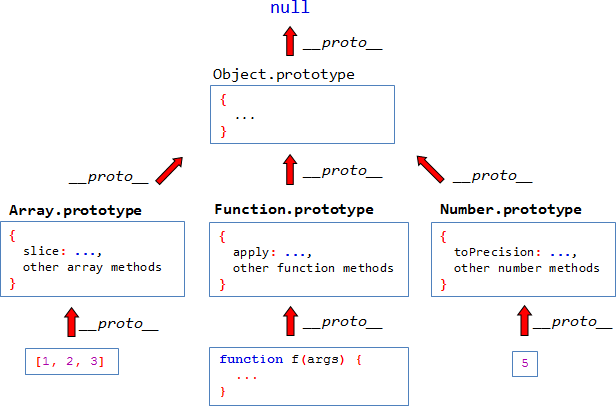
\includegraphics[scale=1.2]{chapter1/javascript_natives.png}
\centerline{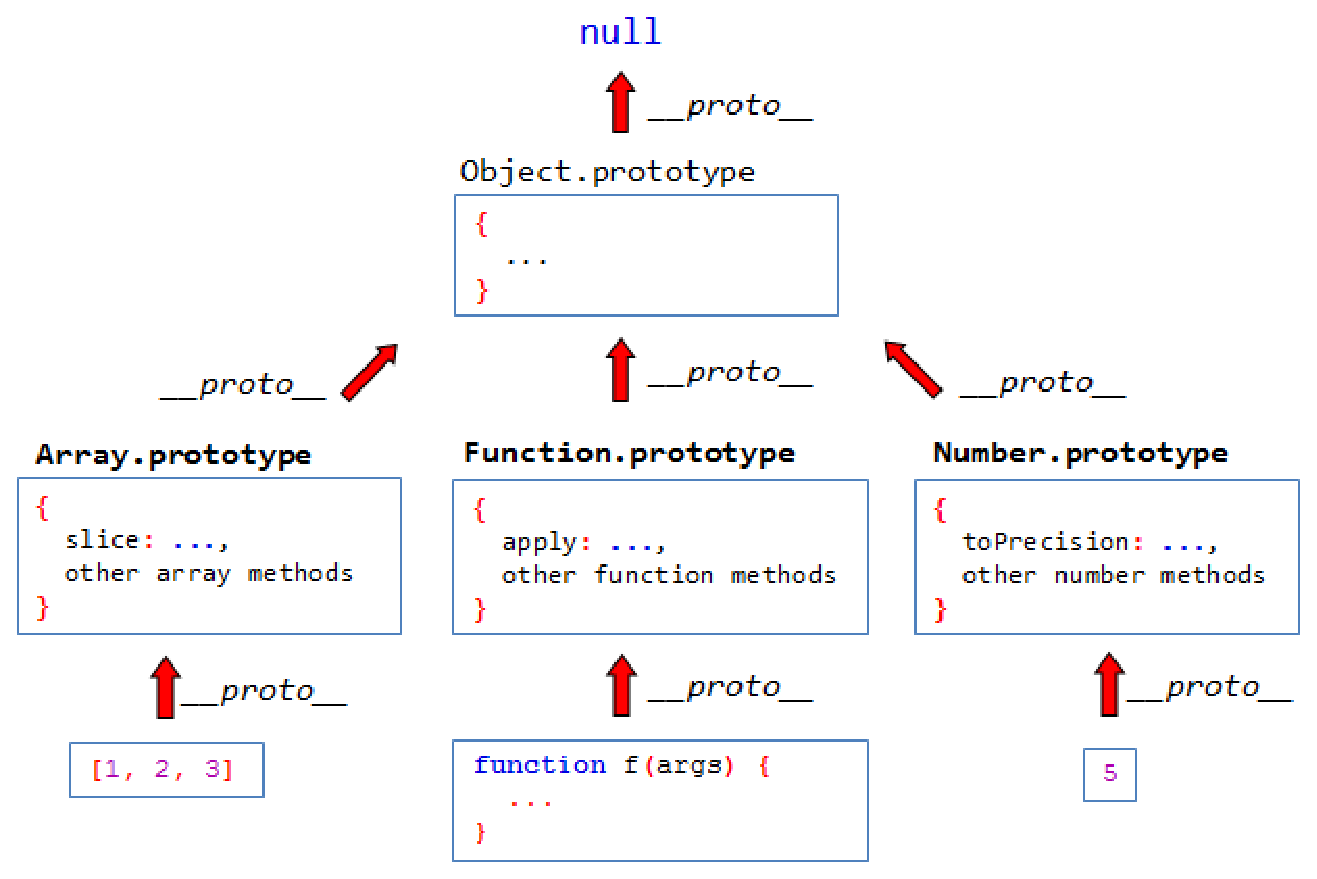
\epsfig{file=chapter1/javascript_natives.eps, width=12cm}}
\end{center}
\label{figure:javascriptnatives}
\caption{Jerarquía de Prototipos Nativos}
\end{figure}

% \begin{figure}[htb]
% \centerline{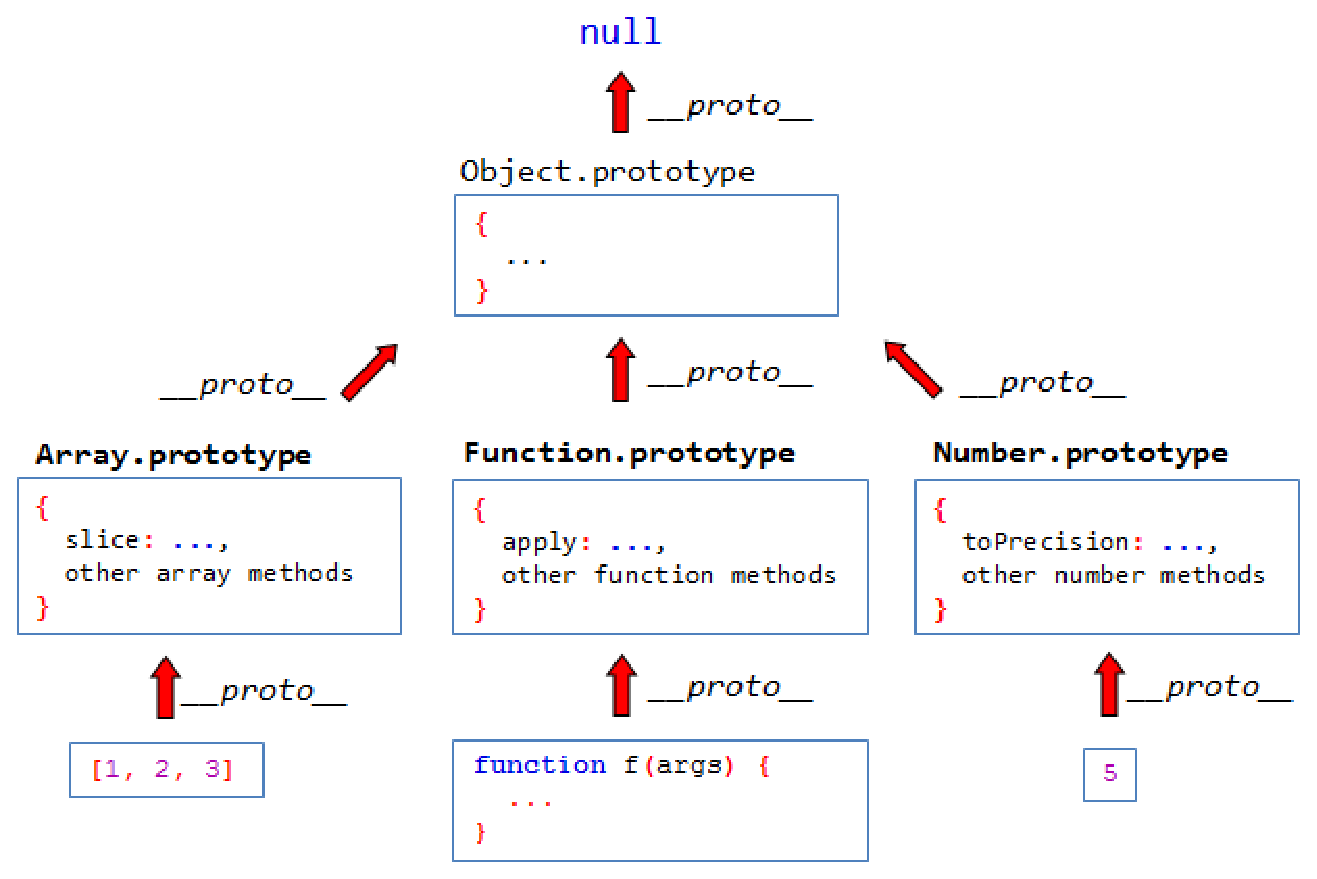
\epsfig{file=chapter1/javascript_natives.eps, height=14cm}}
% \caption{Jerarquía de Prototipos Nativos}
% \label{figure:javascriptnatives}
% \end{figure}

\begin{verbatim}
var b = new Foo(20);
var c = new Foo(30);
\end{verbatim}
\begin{figure}[htb]
\begin{center}
% 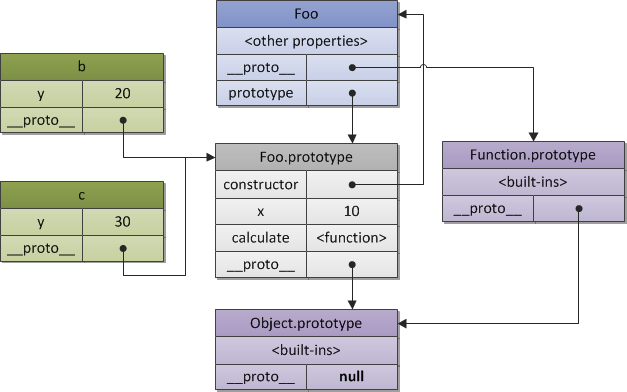
\includegraphics[scale=1]{chapter1/proto_and_prototypes.png}
\centerline{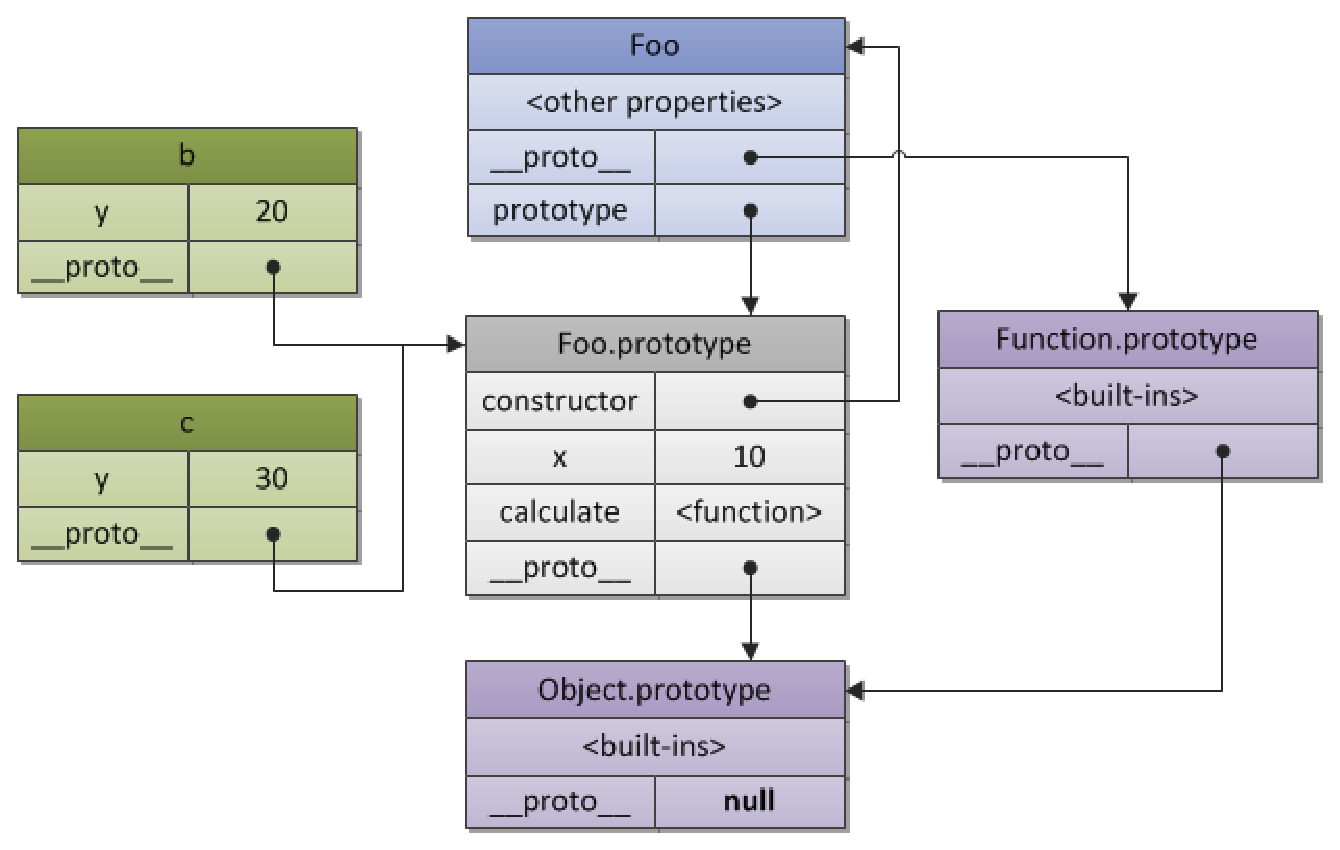
\epsfig{file=chapter1/proto_and_prototypes.eps, width=12cm}}
\end{center}
\label{figure:javascriptnatives}
\caption{\_\_proto\_\_ and prototypes}
\end{figure}

\section{Comprobando Propiedades}

\begin{verbatim}
> o = { x: 1}
{ x: 1 }
> "x" in o
true
> "y" in o
false
> "toString" in o
true
> o.hasOwnProperty('x')
true
> o.hasOwnProperty('toString')
false
\end{verbatim}

\section{Enumeración de Propiedades}

\begin{verbatim}
> o = { x: 1 }
{ x: 1 }
> b = Object.create(o)
{}
> b.y = 2
2
> b.propertyIsEnumerable('x')
false
> b.propertyIsEnumerable('y')
true
> Object.prototype.propertyIsEnumerable('toString')
false
> a = {x:1, y:2 }
{ x: 1, y: 2 }
> b = Object.create(a)
{}
> b.z = 3
3
> for(i in b) console.log(b[i])
3
1
2
undefined
> for(i in b) console.log(i)
z
x
y
undefined
> b.propertyIsEnumerable("toString")
false
\end{verbatim}

\chapter{Arrays}

\chapter{Funciones}
\section{Definiendo Funciones}

\section{Invocando Funciones}

\section{Argumentos y Parámetros}

\section{Funciones como Valores}

\section{Funciones como Espacios de Nombres}

\section{Clausuras}

\section{Propiedades, Métodos y Constructor}

\subsection{La propiedad {\tt length}}

\subsection{La Propiedad {\tt property}}

\subsection{Los Métodos {\tt call} y {\tt apply}}
\label{subsection:callyapply}
Los métodos \tei{call} y \tei{apply} nos permiten
invocar una función como si fuera un método de algún otro 
objeto.

\begin{verbatim}
[~/Dropbox/src/javascript/learning]$ cat call.js 
var Bob = {
  name: "Bob",
  greet: function() {
    console.log("Hi, I'm " + this.name);
  }
}
 
var Alice = {
  name: "Alice",
};

Bob.greet.call(Alice);
\end{verbatim}

\begin{verbatim}
[~/Dropbox/src/javascript/learning]$ node call.js
Hi, I'm Alice
\end{verbatim}

\begin{enumerate}
\item 
\htmladdnormallink{Function.apply and Function.call in JavaScript}{http://odetocode.com/blogs/scott/archive/2007/07/05/function-apply-and-function-call-in-javascript.aspx}
\begin{verbatim}
> function f() { console.log(this.x); }
undefined
> f.toString()
'function f() { console.log(this.x); }'
> z = { x : 99 }
{ x: 99 }
> f.call(z)
99
undefined
> 
\end{verbatim}
\item 
\begin{verbatim}
> o  = { x : 15 }
{ x: 15 }
> function f(m) { console.log(m+" "+this.x); }
undefined
> f("invoking f")
invoking f 10
undefined
> f.call(o, "invoking f via call");
invoking f via call 15
undefined
\end{verbatim}
\end{enumerate}


\section{Programación Funcional}



\chapter{Clases y Módulos}
Véase el libro {\it Learning JavaScript Design Pattern}
\cite{osmani2012learning}

\section{Herencia}

\begin{verbatim}
[~/Dropbox/src/javascript/inheritance]$ cat inh1.js 
//Shape - superclass
function Shape() {
  this.x = 0;
  this.y = 0;
}
 
Shape.prototype.toString = function() {
  return "("+this.x+", "+this.y+")";
}

Shape.prototype.move = function(x, y) {
    this.x += x;
    this.y += y;
    console.info("Shape moved to "+this);
};
 
// Rectangle - subclass
function Rectangle() {
  Shape.call(this); //call super constructor.
}
 
// Rectangle inherits from Shape
Rectangle.prototype = Object.create(Shape.prototype);
 
var rect = new Rectangle();
 
console.log("x = "+rect);
console.log("rect is an instance of Rectangle? "+(rect instanceof Rectangle)) //true.
console.log("rect is an instance of Shape? "+(rect instanceof Shape))         //true.
 
rect.move(1, 2); //Outputs, "Shape moved."
\end{verbatim}

\begin{verbatim}
[~/Dropbox/src/javascript/inheritance]$ node inh1.js 
x = (0, 0)
rect is an instance of Rectangle? true
rect is an instance of Shape? true
Shape moved to (1, 2)

\end{verbatim}

\section{Ejercicios}
\begin{enumerate}
\item ¿Cual es la salida?
\begin{verbatim}
> String.prototype.repeat = function(times) {
...   return new Array(times+1).join(this)
... }
[Function]
>  
undefined
> "hello".repeat(3)

> 
\end{verbatim}

\item  ¿Cuales son los resultados?
\begin{verbatim}
> z = Object.create({x:1, y:2})
{}
> z.x

> z.y

> z.__proto__

> z.__proto__.__proto__

> z.__proto__.__proto__.__proto__

\end{verbatim}
\item 
Describa las salidas:
\begin{verbatim}
> obj = {x : 'something' }
{ x: 'something' }
> w = Object.create(obj)
{}
> w.x
'something'
> w.x = "another thing"
'another thing'
> w.__proto__

> obj == w.__proto__

\end{verbatim}
\item 
Explique la salida:
\begin{verbatim}
> obj = {x : { y : 1} }
{ x: { y: 1 } }
> w = Object.create(obj)
{}
> w.x == obj.x
true
> w.x.y = 2
2
> obj
{ x: { y: 2 } }
> 
\end{verbatim}
\item 
Explique las salidas:
\begin{verbatim}
> inherit = Object.create
[Function: create]
> o = {}
{}
> o.x = 1
1
> p = inherit(o)
{}
> p.x
1
> p.y = 2
2
> p
{ y: 2 }
> o
{ x: 1 }
> o.y
undefined
> q = inherit(p)
{}
> q.z = 3
3
> q
{ z: 3 }
> s = q.toString()
'[object Object]'
> q.x+q.y+q.z
6
> o.x
1
> o.x = 4
4
> p.x
4
> q.x
4
> q.x = 5
5
> p.x
4
> o.x
4
\end{verbatim}
\end{enumerate}


\chapter{Subconjuntos y Extensiones de JavaScript}

\chapter{JavaScript en el Lado del Servidor}
Node es un intérprete JavScript escrito en C++ y con una API ligada a
Unix para trabajar con procesos, fichero, sockets, etc.  Los programas
Node por defecto nunca se bloquean. Node utiliza manejadores de eventos
que a menudo se implementan haciendo uso de funciones anidadas  y
clausuras.


\section{Instalar Node.js}
\begin{enumerate}
\item \htmladdnormallink{http://nodejs.org/download/}{http://nodejs.org/download/}
\item 
\htmladdnormallink{Should I install node.js on Ubuntu using package manager or from source?}{http://stackoverflow.com/questions/13845321/should-i-install-node-js-on-ubuntu-using-package-manager-or-from-source}
\item 
\htmladdnormallink{The Node Beginner Book}{http://www.nodebeginner.org/}
\end{enumerate}


\section{Primeros Pasos. Un Ejemplo Simple}
\begin{verbatim}
[~/src/javascript/node.js/hector_correa_introduction_to_node(master)]$ cat -n hello_world.js 
     1  console.log("Hello world!");
     2  a = [ 'batman', 'robin'];
     3  a.push("superman");
     4  console.log(a);
     5  h = { name: 'jane rodriguez-leon', department: 'IT' };
     6  console.log(h);
     7  console.log(h['name']);
\end{verbatim}

\begin{verbatim}
[~/src/javascript/node.js/hector_correa_introduction_to_node(master)]$ node hello_world.js 
Hello world!
[ 'batman', 'robin', 'superman' ]
{ name: 'jane rodriguez-leon', department: 'IT' }
jane rodriguez-leon
\end{verbatim}

\begin{verbatim}
[~/Dropbox/academica/ETSII/grado/LPP/LPPbook]$ node
> .help
.break  Sometimes you get stuck, this gets you out
.clear  Alias for .break
.exit Exit the repl
.help Show repl options
.load Load JS from a file into the REPL session
.save Save all evaluated commands in this REPL session to a file

> console.log("Hello world!")
Hello world!
undefined
> a = [ 'batman', 'robin']
[ 'batman', 'robin' ]
> a.push("superman")
3
> a
[ 'batman', 'robin', 'superman' ]
> h = { name: 'jane rodriguez-leon', department: 'IT' }
{ name: 'jane rodriguez-leon',
  department: 'IT' }
> h['name']
'jane rodriguez-leon'
> 4+2
6
> _    # ultimo valor evaluado
6
> _+1
7
> 
> a = [1,2,3]
[ 1, 2, 3 ]
> a.forEach(function(e) { console.log(e); })
1
2
3
> a.forEach(function(v) {
... console.log(v
..... .break
> a
[ 1, 2, 3 ]
> .exit # también CTRL-D en Unix
[~/Dropbox/academica/ETSII/grado/LPP/LPPbook]$ 
\end{verbatim}

\section{Usando REPL desde un programa}

Es posible crear un bucle REPL en cualquier punto de nuestro programa - quizá para depurarlo.
Para ello usamos la función 
\tei{repl.start}.
Esta función retorna una instancia REPLServer. Acepta como argumento un objeto
\verb"options" que toma los siguientes valores:

\begin{enumerate}
\item \verb|prompt| - the prompt and stream for all I/O. Defaults to > .
\item \verb|input| - the readable stream to listen to. Defaults to process.stdin.
\item \verb|output| - the writable stream to write readline data to. Defaults to process.stdout.
\item \verb|terminal| - pass true if the stream should be treated
like a TTY, and have ANSI/VT100 escape codes written to it. Defaults
to checking isTTY on the output stream upon instantiation.
\item \verb|eval| - function that will be used to eval each given
line. Defaults to an async wrapper for eval(). 
\item \verb|useColors| - a boolean which specifies whether or not
the writer function should output colors. If a different writer
function is set then this does nothing. Defaults to the repl's
terminal value.
\item \verb|useGlobal| - if set to true, then the repl will use the
global object, instead of running scripts in a separate context.
Defaults to false.
\item \verb|ignoreUndefined| - if set to true, then the repl will
not output the return value of command if it's undefined. Defaults
to false.
\item \verb|writer| - the function to invoke for each command that
gets evaluated which returns the formatting (including coloring)
to display. Defaults to util.inspect.
\end{enumerate}

\begin{verbatim}
[~/Dropbox/src/javascript/node.js/repl(master)]$ cat repl.js 
var repl = require("repl");

connections = 0;

repl.start({
  prompt: "node via stdin> ",
  input: process.stdin,
  output: process.stdout
});
\end{verbatim}

\begin{verbatim}
[~/Dropbox/src/javascript/node.js/repl(master)]$ node repl.js 
node via stdin> 2+3
5
node via stdin> .exit
\end{verbatim}

el bucle REPL proporciona acceso a las variables de ámbito global. Es posible
hacer explícitamente visible una variable al REPL asignándosela al
\verb|context| asociado con el
REPLServer. Por ejemplo:

\begin{verbatim}
[~/Dropbox/src/javascript/node.js/repl(master)]$ cat repl2.js 
var repl = require("repl");

z = 4
repl.start({
  prompt: "node via stdin> ",
  input: process.stdin,
  output: process.stdout
}).context.m = "message";
\end{verbatim}
Las variables en el objeto \verb|context| se ven como locales 
al  REPL:

\begin{verbatim}
[~/Dropbox/src/javascript/node.js/repl(master)]$ node repl2.js 
node via stdin> z
4
node via stdin> m
'message'

\end{verbatim}

\section{Usando REPL via un socket TCP}
\begin{verbatim}
[~/Dropbox/src/javascript/node.js/repl(master)]$ cat repl_server.js 
var net = require("net"),
    repl = require("repl");

connections = 0;

net.createServer(function (socket) {
  connections += 1;
  repl.start({
    prompt: "node via TCP socket> ",
    input: socket,
    output: socket
  }).on('exit', function() {
    socket.end();
  });
}).listen(5001);

[~/Dropbox/src/javascript/node.js/repl(master)]$ node repl_server.js 

\end{verbatim}

Podemos ahora usar \cei{netcat} para comunicar con el servidor:
\begin{verbatim}
[~/Dropbox/src/javascript/node.js/hector_correa_introduction_to_node(master)]$ nc -v localhost 5001
nc: connect to localhost port 5001 (tcp) failed: Connection refused
Connection to localhost 5001 port [tcp/commplex-link] succeeded!
node via TCP socket> a = 2+3
5
node via TCP socket> a
5
node via TCP socket> .exit
[~/Dropbox/src/javascript/node.js/hector_correa_introduction_to_node(master)]$ 
\end{verbatim}

\section{Referencias sobre REPL}

\begin{enumerate}
\item 
Véase \htmladdnormallink{Node.js v0.8.18 Manual \& Documentation}{http://nodejs.org/api/repl.html}
\item 
Véase \htmladdnormallink{How do I use node's REPL?}{http://docs.nodejitsu.com/articles/REPL/how-to-use-nodejs-repl} en \htmladdnormallink{http://docs.nodejitsu.com/}{http://docs.nodejitsu.com/}.
\end{enumerate}

\section{Entrada Salida en Node.js}

\begin{enumerate}
\item 
\htmladdnormallink{How To Read User Input With NodeJS}{http://st-on-it.blogspot.com.es/2011/05/how-to-read-user-input-with-nodejs.html} por Nikolay V. Nemshilov
\end{enumerate}

\section{Debugger}

\begin{enumerate}
\item 
\htmladdnormallink{Node.js debugger}{http://nodejs.org/api/debugger.html}
\end{enumerate}

\section{Modulos}
%http://nodejs.org/api/modules.html#loading_from_node_modules_Folders
\subsection{Introducción}

\begin{verbatim}
[~/javascript/node.js/creating_modules(master)]$ cat foo.js 
var circle = require('./circle.js');
console.log( 'The area of a circle of radius 4 is '
           + circle.area(4));
\end{verbatim}

\begin{verbatim}
[~/javascript/node.js/creating_modules(master)]$ cat circle.js 
var PI = Math.PI;

exports.area = function (r) {
  return PI * r * r;
};

exports.circumference = function (r) {
  return 2 * PI * r;
};
\end{verbatim}

\begin{verbatim}
[~/javascript/node.js/creating_modules(master)]$ node foo.js The area of a circle of radius 4 is 50.26548245743669
\end{verbatim}

El módulo \verb|circle.js| exporta las funciones \verb|area()| 
y \verb|circumference()|. Para exportar un objeto lo añadimos 
al objeto expecial \verb|exports|.

Las variables locales al módulo serán privadas.
En este ejemplo la variable \verb|PI| es privada a \verb|circle.js|.

\begin{verbatim}
[~/javascript/node.js/creating_modules(master)]$ node debug foo.js 
< debugger listening on port 5858
connecting... ok
break in foo.js:1
  1 var circle = require('./circle.js');
  2 console.log( 'The area of a circle of radius 4 is '
  3            + circle.area(4));
debug> n
break in foo.js:2
  1 var circle = require('./circle.js');
  2 console.log( 'The area of a circle of radius 4 is '
  3            + circle.area(4));
  4 
debug> repl
Press Ctrl + C to leave debug repl
> circle
{ circumference: [Function],
  area: [Function] }
> circle.area(2)
12.566370614359172
> PI
ReferenceError: PI is not defined
> 
\end{verbatim}

\subsection{Ciclos}

\begin{verbatim}
[~/javascript/node.js/creating_modules/cycles(master)]$ cat a.js
console.log('a starting');
exports.done = false;
var b = require('./b.js');
console.log('in a, b.done = %j', b.done);
exports.done = true;
console.log('a done');
\end{verbatim}

\begin{verbatim}
[~/javascript/node.js/creating_modules/cycles(master)]$ cat b.js
console.log('b starting');
exports.done = false;
var a = require('./a.js');
console.log('in b, a.done = %j', a.done);
exports.done = true;
console.log('b done');
\end{verbatim}

\begin{verbatim}
[~/javascript/node.js/creating_modules/cycles(master)]$ cat main.js
console.log('main starting');
var a = require('./a.js');
var b = require('./b.js');
console.log('in main, a.done=%j, b.done=%j', a.done, b.done);
\end{verbatim}
When \verb|main.js| loads \verb|a.js|, then \verb|a.js| in turn loads
\verb|b.js|. At that point, \verb|b.js| tries to load \verb|a.js|. In
order to prevent an infinite loop an unfinished copy of the \verb|a.js|
exports object is returned to the \verb|b.js| module. \verb|b.js| then
finishes loading, and its exports object is provided to the \verb|a.js|
module.

By the time \verb|main.js| has loaded both modules, they're both finished. The
output of this program would thus be:

\begin{verbatim}
[~/javascript/node.js/creating_modules/cycles(master)]$ node main.js 
main starting
a starting
b starting
in b, a.done = false
b done
in a, b.done = true
a done
in main, a.done=true, b.done=true
\end{verbatim}

\subsection{Especificación de Ficheros Conteniendo Módulos}

\begin{enumerate}
\item If the exact filename is not found, then node will attempt to
load the required filename with the added extension of \verb|.js|,
\verb|.json|, and then \verb|.node|.

\item
\verb|.js| files are interpreted as JavaScript text files, and \verb|.json| files are parsed as JSON text files. \verb|.node| files are interpreted as compiled addon modules 

\item
A module prefixed with \verb|'/'| is an absolute path to the file. For example,
\verb|require('/home/marco/foo.js')| will load the file at \verb|/home/marco/foo.js|.

\item
A module prefixed with \verb|'./'| is relative to the file calling require(). 

\item
Without a leading verb|'/'| or \verb|'./'| to indicate a file, the module is either a 
\cei{core module} or is loaded from a \verb|node_modules| folder.

\item
If the given path does not exist, \verb|require()| 
will throw an Error with its code property set to \verb'MODULE_NOT_FOUND'.
\end{enumerate}

\subsection{Carga desde Carpetas {\tt node\_modules}}

\begin{enumerate}
\item
If the module identifier passed to \verb|require()| is not a native module,
and does not begin with \verb|'/'|, \verb|'../'|, or \verb|'./'|, then node starts at the
parent directory of the current module, and adds \verb|/node_mo1dules|, and
attempts to load the module from that location.

\item
If it is not found there, then it moves to the parent directory, and so
on, until the root of the tree is reached.
\end{enumerate}

For example, if the file at \verb|'/home/ry/projects/foo.js'| called
require(\verb|'bar.js'|), then node would look in the following locations,
in this order:

\begin{verbatim}
/home/ry/projects/node_modules/bar.js
/home/ry/node_modules/bar.js
/home/node_modules/bar.js
/node_modules/bar.js
\end{verbatim}

This allows programs to localize their dependencies, so that they do not clash.

\subsection{Las Carpetas Usadas Como Módulos}
It is convenient to organize programs and libraries into self-contained
directories, and then provide a single entry point to that library. 

There
are a few ways in which a folder may be passed to \verb|require()| as an
argument.

\begin{enumerate}
\item
The first is to create a \verb|package.json| file in the root of the
folder, which specifies a \verb|main| module. 
An example \verb|package.json| file
might look like this:

\begin{verbatim}
{ "name" : "some-library",
  "main" : "./lib/some-library.js" }
\end{verbatim}

If this was in a folder at 
\verb|./some-library|, then \verb|require('./some-library')| would attempt
to load \verb|./some-library/lib/some-library.js|.

This is the extent of Node's awareness of \verb|package.json| files.

\item
If there is no \verb|package.json| 
file present in the directory, then node will
attempt to load an 
\verb|index.js| or
\verb|index.node| 
file out of that directory. 

For
example, if there was no 
\verb|package.json| file in the above example, then
\verb|require('./some-library')| would attempt to load:

\begin{verbatim}
./some-library/index.js
./some-library/index.node
\end{verbatim}

\end{enumerate}

\subsection{Caching}

\begin{enumerate}
\item
Modules are cached after the first time they are loaded. This means
(among other things) that every call to \verb|require('foo')| will get exactly
the same object returned, if it would resolve to the same file.

\item
Multiple calls to \verb|require('foo')| may not cause the module code
to be executed multiple times. This is an important feature. With it,
\cei{partially done} objects can be returned, thus allowing transitive
dependencies to be loaded even when they would cause cycles.

\item
If you want to have a module execute code multiple times, then export
a function, and call that function.

\item
Modules are cached based on their {\bf resolved filename}. Since modules may
resolve to a different filename based on the location of the calling
module (loading from \verb|node_modules folders|), it is not a guarantee that
\verb|require('foo')| will always return the exact same object, if it would
resolve to different files.

\end{enumerate}

\subsection{El Objeto {\tt module} y {\tt module.exports}}

\begin{enumerate}
\item
In each module, the \verb|module| free variable is a reference to the object
representing the current module. 

\item
In particular \verb|module.exports| is the
same as the exports object. 

\item
\verb|module| isn't actually a global but rather
local to each module.

\item
The exports object is created by the \verb|Module| system. 
Sometimes this is not acceptable, 
many want their module to be an instance of some class. 
To do this assign the desired export object to \verb|module.exports|. 

\begin{itemize}
\item
\begin{verbatim}
[~/javascript/node.js/creating_modules/module_exports(master)]$ cat a.js
var EventEmitter = require('events').EventEmitter;

module.exports = new EventEmitter();

// Do some work, and after some time emit
// the 'ready' event from the module itself.
setTimeout(function() {
  module.exports.emit('ready');
}, 1000);
\end{verbatim}

\item
\begin{verbatim}
$ cat main.js 
var a = require('./a');
a.on('ready', function() {
  console.log('module a is ready');
});
\end{verbatim}
\item
\begin{verbatim}
$ node main.js 
module a is ready
\end{verbatim}
\end{itemize}
La asignación a \verb|module.exports| debe hacerse inmediatamente. 
No puede hacerse en un callback.

\end{enumerate}

\subsection{Algoritmo de Búsqueda Ejecutado por {\tt require}}

\parrafo{require(X) from module at path Y}
\begin{enumerate}
\item If X is a core module,
\begin{enumerate}
  \item return the core module
  \item STOP
\end{enumerate}
\item If X begins with './' or '/' or '../'
\begin{enumerate}
  \item \verb|LOAD_AS_FILE(Y + X)|
  \item \verb|LOAD_AS_DIRECTORY(Y + X)|
\end{enumerate}
\item \verb|LOAD_NODE_MODULES(X, dirname(Y))|
\item THROW "not found"
\end{enumerate}

\parrafo{LOAD\_AS\_FILE(X)}
\begin{enumerate}
\item If X is a file, load X as JavaScript text.  STOP
\item If X.js is a file, load X.js as JavaScript text.  STOP
\item If X.node is a file, load X.node as binary addon.  STOP
\end{enumerate}

\parrafo{LOAD\_AS\_DIRECTORY(X)}
\begin{enumerate}
\item If X/package.json is a file,
   a. Parse X/package.json, and look for "main" field.
   b. let M = X + (json main field)
   c. \verb|LOAD_AS_FILE(M)|
\item If X/index.js is a file, load X/index.js as JavaScript text.  STOP
\item If X/index.node is a file, load X/index.node as binary addon.  STOP
\end{enumerate}

\parrafo{LOAD\_NODE\_MODULES(X, START)}
\begin{enumerate}
\item let \verb|DIRS=NODE_MODULES_PATHS(START)|
\item for each DIR in DIRS:
   a. \verb|LOAD_AS_FILE(DIR/X)|
   b. \verb|LOAD_AS_DIRECTORY(DIR/X)|
\end{enumerate}

\parrafo{NODE\_MODULES\_PATHS(START)}
\begin{enumerate}
\item let PARTS = path split(START)
\item let ROOT = index of first instance of "node\_modules" in PARTS, or 0
\item let I = count of PARTS - 1
\item let DIRS = []
\item while I > ROOT,
   a. if PARTS[I] = "node\_modules" CONTINUE
   c. DIR = path join(PARTS[0 .. I] + "node\_modules")
   b. DIRS = DIRS + DIR
   c. let I = I - 1
\item return DIRS
\end{enumerate}


\section{Como Crear tu Propio Módulo en Node.js}
% http://howtonode.org/how-to-module está desactualizado

\subsection{Introducción}

Cuando Node carga nuestro fichero JavaScript
crea un nuevo ámbito. Cuando estamos en nuestro módulo, no podemos
ver el ámbito externo lo que evita las colisiones de nombres.

\subsection{Un Fichero {\tt package.json}}

Creamos un fichero en la raíz de nuestro proyecto con nombre 
\verb|package.json|. Este fichero describe nuestro proyecto.
Es esencial si vamos a publicar nuestro proyecto con 
\npm{}.

Podemos especificar en este fichero:

\begin{enumerate}
\item
Name, version, description, and keywords to describe your program.
\item
A homepage where users can learn more about it.
\item
Other packages that yours depends on.
\end{enumerate}

Si hemos instalado \npm{} podemos usar el comando 
\verb|npm| \npmdoc{init} para empezar.
Véase  \verb|npm help|
\npmdoc{json} 
para obtener información sobre este fichero:

La cosa mas importante a especificar 
cuando estamos escribiendo un programa para su uso por otros,
es el módulo \verb|main|. Este consituirá el punto de entrada 
a nuestro programa.

Es esencial documentar las dependencias.

El siguiente es un ejemplo de fichero \verb|package.json| tomado
del proyecto \ebnfparser{}:
\begin{verbatim}
[~/javascript/PLgrado/ebnf-parser(master)]$ cat -n package.json 
   1  {
   2    "name": "ebnf-parser",
   3    "version": "0.1.1",
   4    "description": "A parser for BNF and EBNF grammars used by jison",
   5    "main": "ebnf-parser.js",
   6    "scripts": {
   7      "test": "make test"
   8    },
   9    "repository": "",
  10    "keywords": [
  11      "bnf",
  12      "ebnf",
  13      "grammar",
  14      "parser",
  15      "jison"
  16    ],
  17    "author": "Zach Carter",
  18    "license": "MIT",
  19    "devDependencies": {
  20      "jison": "0.4.x",
  21      "lex-parser": "0.1.0",
  22      "test": "*"
  23    }
  24  }
\end{verbatim}

\subsection{README y otros documentos}

Pon la información basica acerca del módulo 
en la raíz del proyecto.
Como ejemplo veamos el \verb|README.md| (observa que 
está en formato \markdown{}) 
del proyecto \ebnfparser{}:

\begin{verbatim}
$ cat README.md 

# ebnf-parser

A parser for BNF and EBNF grammars used by jison.

## install

    npm install ebnf-parser


## build

To build the parser yourself, clone the git repo then run:

    make

This will generate `parser.js`, which is required by `ebnf-parser.js`.

## usage

The parser translates a string grammar or JSON grammar into a JSON grammar that jison can use (ENBF is transformed into BNF).

    var ebnfParser = require('ebnf-parser');

    // parse a bnf or ebnf string grammar
    ebnfParser.parse("%start ... %");

    // transform an ebnf JSON gramamr
    ebnfParser.transform({"ebnf": ...});


## example grammar

The parser can parse its own BNF grammar, shown below:

    %start spec

    /* grammar for parsing jison grammar files */

    %{
    var transform = require('./ebnf-transform').transform;
    var ebnf = false;
    %}

    %%

    spec
        : declaration_list '%%' grammar optional_end_block EOF
            {$$ = $1; return extend($$, $3);}
        | declaration_list '%%' grammar '%%' CODE EOF
            {$$ = $1; yy.addDeclaration($$,{include:$5}); return extend($$, $3);}
        ;

    optional_end_block
        :
        | '%%'
        ;

    declaration_list
        : declaration_list declaration
            {$$ = $1; yy.addDeclaration($$, $2);}
        |
            {$$ = {};}
        ;

    declaration
        : START id
            {$$ = {start: $2};}
        | LEX_BLOCK
            {$$ = {lex: $1};}
        | operator
            {$$ = {operator: $1};}
        | ACTION
            {$$ = {include: $1};}
        ;

    operator
        : associativity token_list
            {$$ = [$1]; $$.push.apply($$, $2);}
        ;

    associativity
        : LEFT
            {$$ = 'left';}
        | RIGHT
            {$$ = 'right';}
        | NONASSOC
            {$$ = 'nonassoc';}
        ;

    token_list
        : token_list symbol
            {$$ = $1; $$.push($2);}
        | symbol
            {$$ = [$1];}
        ;

    grammar
        : production_list
            {$$ = $1;}
        ;

    production_list
        : production_list production
            {$$ = $1;
              if($2[0] in $$) $$[$2[0]] = $$[$2[0]].concat($2[1]);
              else  $$[$2[0]] = $2[1];}
        | production
            {$$ = {}; $$[$1[0]] = $1[1];}
        ;

    production
        : id ':' handle_list ';'
            {$$ = [$1, $3];}
        ;

    handle_list
        : handle_list '|' handle_action
            {$$ = $1; $$.push($3);}
        | handle_action
            {$$ = [$1];}
        ;

    handle_action
        : handle prec action
            {$$ = [($1.length ? $1.join(' ') : '')];
                if($3) $$.push($3);
                if($2) $$.push($2);
                if ($$.length === 1) $$ = $$[0];
            }
        ;

    handle
        : handle expression_suffix
            {$$ = $1; $$.push($2)}
        |
            {$$ = [];}
        ;

    handle_sublist
        : handle_sublist '|' handle
            {$$ = $1; $$.push($3.join(' '));}
        | handle
            {$$ = [$1.join(' ')];}
        ;

    expression_suffix
        : expression suffix
            {$$ = $expression + $suffix; }
        ;

    expression
        : ID
            {$$ = $1; }
        | STRING
            {$$ = ebnf ? "'"+$1+"'" : $1; }
        | '(' handle_sublist ')'
            {$$ = '(' + $handle_sublist.join(' | ') + ')'; }
        ;

    suffix
        : {$$ = ''}
        | '*'
        | '?'
        | '+'
        ;

    prec
        : PREC symbol
            {$$ = {prec: $2};}
        |
            {$$ = null;}
        ;

    symbol
        : id
            {$$ = $1;}
        | STRING
            {$$ = yytext;}
        ;

    id
        : ID
            {$$ = yytext;}
        ;

    action
        : '{' action_body '}'
            {$$ = $2;}
        | ACTION
            {$$ = $1;}
        | ARROW_ACTION
            {$$ = '$$ ='+$1+';';}
        |
            {$$ = '';}
        ;

    action_body
        :
            {$$ = '';}
        | ACTION_BODY
            {$$ = yytext;}
        | action_body '{' action_body '}' ACTION_BODY
            {$$ = $1+$2+$3+$4+$5;}
        | action_body '{' action_body '}'
            {$$ = $1+$2+$3+$4;}
        ;

    %%

    // transform ebnf to bnf if necessary
    function extend (json, grammar) {
        json.bnf = ebnf ? transform(grammar) : grammar;
        return json;
    }

## license

MIT
\end{verbatim}

En general se anima  a que uses el formato markdown. Salva el fichero como
\verb|README.md|.

La documentación adicional se pone en un directorio \verb|./docs|. 
Los ficheros markdown teminan en \verb|.md| y los html en \verb|.html|.

\subsection{Véase También}
\begin{itemize}
\item
\htmladdnormallink{How To: Create Your Own Node.js Module}{http://howtonode.org/how-to-module} por Isaac Z. Schlueter autor de 
\htmladdnormallink{npm}{http://npmjs.org/}.
Véase también este
\htmladdnormallink{gist en GitHub}{https://gist.github.com/isaacs/4150d972e0aa2a4060c1}
\item
\htmladdnormallink{Creating Custom Modules}{http://howtonode.org/creating-custom-modules}
\item
\htmladdnormallink{How to Build a Nodejs Npm Package From Scratch.}{http://decodize.com/javascript/build-nodejs-npm-installation-package-scratch/} May 2012 Decodize

\end{itemize}



\section{Mas sobre Node}
\begin{enumerate}
\item
Véase el libro 'Learning Node' de S. Powers \cite{learningnode}.
\item \htmladdnormallink{Node.js}{http://nodejs.org/}
\item \htmladdnormallink{docs.nodejitsu.com}{http://docs.nodejitsu.com}: collection of node.js how-to articles. These articles range from basic to advanced. They provide relevant code samples and insights into the design and philosophy of node itself

\item \htmladdnormallink{http://howtonode.org/}{http://howtonode.org/}
contiene un número creciente de tutoriales
\item El manual de node.js puede encontrarse en formato pdf en el proyecto 
\htmladdnormallink{https://github.com/zeMirco/nodejs-pdf-docs}{https://github.com/zeMirco/nodejs-pdf-docsoen}
en GitHub. En concreto en este \htmladdnormallink{enlace}{https://github.com/zeMirco/nodejs-pdf-docs/blob/master/pdf/all.pdf?raw=true}
\item \htmladdnormallink{Guías de node.js}{http://nodeguide.com/} de
\htmladdnormallink{Felix Geisendörfer}{https://twitter.com/felixge}
\item \htmladdnormallink{Introduction to Node.js}{http://hectorcorrea.jit.su/blog/introduction-to-node-js} por Hector Correa
\item \htmladdnormallink{El Libro para Principiantes en Node.js}{http://www.nodebeginner.org/index-es.html} por Manuel Kiessling  y Herman A. Junge
\end{enumerate}
Para aprender JavaScript podemos usar el libro
\htmladdnormallink{eloquent JavaScript}{http://eloquentjavascript.net/} de Marijn Haverbeke \cite{eloquentjavascript}.




\chapter{JavaScript en los Navegadores}

\chapter{El Objeto Window}

\chapter{Manejo de Documentos en JavaScript}


\chapter{Manejo de Eventos}



\chapter{La Librería JQuery}

\chapter{Almacenamiento en el Cliente}

\chapter{Multimedia y Gráficos}


\chapter{Backbone}
\begin{enumerate}
\item 
\htmladdnormallink{Developing Backbone.js Applications}{http://addyosmani.github.com/backbone-fundamentals/}
\end{enumerate}

\chapter{Closure Tools}

\section{Véase También}
\begin{enumerate}
\item
\htmladdnormallink{Google I/O 2011: JavaScript Programming in the Large with Closure Tools}{http://youtu.be/M3uWx-fhjUc}  (YouTube)
\item
\htmladdnormallink{The Closure Tools project is an effort by Google to open source the tools used in many of Google's sites and web applications}{https://developers.google.com/closure/?hl=es}
\item Herramientas:
\begin{enumerate}
\item
\htmladdnormallink{Closure Compiler}{https://code.google.com/p/closure-compiler/} en Google-Code
\item
\htmladdnormallink{Closure Library}{https://code.google.com/p/closure-library/} en Google-Code
\item
\htmladdnormallink{Closure Template}{https://code.google.com/p/closure-templates/} en Google-Code
\item
\htmladdnormallink{Closure Linter}{https://code.google.com/p/closure-linter/} en Google-Code
\end{enumerate}
\item
\htmladdnormallink{Getting Started with the Closure Library}{https://developers.google.com/closure/library/docs/gettingstarted?hl=es} (Hello World!)
\end{enumerate}



\chapter{Semantic Templates}

\section{Moustache}

\begin{itemize}
\item
\htmladdnormallink{http://mustache.github.io/}{http://mustache.github.io/}
\item
\htmladdnormallink{Tutorial: HTML Templates with Mustache.js}{http://coenraets.org/blog/2011/12/tutorial-html-templates-with-mustache-js/}
\end{itemize}

\chapter{Pruebas}
\section{Testing en JavaScript: Fácil y Rápido}
\label{section:tstingfacil}
\begin{enumerate}
\item 
\htmladdnormallink{Quick Tip: Quick and Easy JavaScript Testing with “Assert”}{http://net.tutsplus.com/tutorials/javascript-ajax/quick-tip-quick-and-easy-javascript-testing-with-assert/}
por
\htmladdnormallink{Jeffrey Way}{http://net.tutsplus.com/author/jeffreyway/}

\end{enumerate}

\section{Unit Testing, TDD y BDD con Jasmine}
\begin{enumerate}
\item
\htmladdnormallink{Jasmine: BDD Style JavaScript Testing Hello World}{http://youtu.be/nH1Amt_JHLg} por Chris McNabb (YouTube Sep. 2012)
\item
\htmladdnormallink{Download Jasmine}{https://github.com/pivotal/jasmine/downloads}
\item
\htmladdnormallink{Testing Your JavaScript with Jasmine
Andrew Burgess on Aug 4th 2011}{http://net.tutsplus.com/tutorials/javascript-ajax/testing-your-javascript-with-jasmine/?search_index=3}
\item 
\htmladdnormallink{Unit Testing in JavaScript via Jasmine}{http://youtu.be/eVpXkyN0zOE} (Youtube)
\item 
\htmladdnormallink{Jasmine}{http://pivotal.github.com/jasmine/} en GitHub
\item
\htmladdnormallink{Behavior Driven Testing with Jasmine}{http://youtu.be/KdCQFFHUpi4} (YouTube, Davis Frank de Pivotal Labs, Contiene una introducción a BDD)
\item
\htmladdnormallink{Jasmine Wiki}{https://github.com/pivotal/jasmine/wiki}
\item
\htmladdnormallink{Testem}{http://net.tutsplus.com/tutorials/javascript-ajax/make-javascript-testing-fun-with-testem} tutorial en net.tutplus (trabaja sobre Jasmine y sobre Coffee)
\item
Jasmine Matchers: \htmladdnormallink{Class jasmine.Matchers}{http://pivotal.github.com/jasmine/jsdoc/symbols/jasmine.Matchers.html}
\end{enumerate}



\chapter{Buenas Prácticas y Patrones}

\section{Véase También}
\begin{enumerate}
\item
\htmladdnormallink{Google I/O 2011: Learning to Love JavaScript}{http://youtu.be/seX7jYI96GE}
por Alex Russell, Mayo 2011. ¡Excelente!
\item
\htmladdnormallink{traceur compiler}{https://code.google.com/p/traceur-compiler/}
\item
\htmladdnormallink{Google I/O 2011: JavaScript Programming in the Large with Closure Tools}{http://youtu.be/M3uWx-fhjUc} 
\end{enumerate}


\chapter{Herramientas}
\section{npm}

\begin{verbatim}
\end{verbatim}

\section{n}

\tei{n} es una herramienta parecida a \tei{rvm} para Node.js:
\begin{verbatim}
$sudo npm install n -g
\end{verbatim}
y

\begin{verbatim}
[~/Dropbox/src/javascript/node.js/creating_modules(master)]$ n help

  Usage: n [options] [COMMAND] [config]

  Commands:

    n                            Output versions installed
    n latest [config ...]        Install or activate the latest node release
    n stable [config ...]        Install or activate the latest stable node release
    n <version> [config ...]     Install and/or use node <version>
    n use <version> [args ...]   Execute node <version> with [args ...]
    n bin <version>              Output bin path for <version>
    n rm <version ...>           Remove the given version(s)
    n prev                       Revert to the previously activated version
    n --latest                   Output the latest node version available
    n --stable                   Output the latest stable node version available
    n ls                         Output the versions of node available

  Options:

    -V, --version   Output current version of n
    -h, --help      Display help information

  Aliases:

    which   bin
    use     as
    list    ls
    -       rm
\end{verbatim}

\begin{verbatim}
$ sudo n latest
\end{verbatim}

\section{Karma}
\label{subsection:karma}
\subsection{Preguntas de Repaso de
Karma}\label{preguntas-de-repaso-de-karma}

\begin{enumerate}
\def\labelenumi{\arabic{enumi}.}
\item
  Explique como funciona Karma
\item
  ¿Con que comando puedo crear el fichero de configuración de Karma?
\item
  ¿Que debemos poner en la entrada \texttt{frameworks} de karma para el
  ejemplo de la temperatura?

\begin{verbatim}
    frameworks: ['_____'],
\end{verbatim}
\item
  La librería/plugin \texttt{karma-mocha} provee el adapter de Karma
  para Mocha. ¿Como le pasamos opciones para configurar Mocha desde
  Karma? Rellene las partes que faltan:
\end{enumerate}

\begin{Shaded}
\begin{Highlighting}[]
\NormalTok{client: \{}
  \DataTypeTok{args}\NormalTok{: [}\StringTok{'--grep'}\NormalTok{, }\StringTok{'pattern'}\NormalTok{], }\CommentTok{// solo pruebas que casan con pattern}
  \DataTypeTok{mocha}\NormalTok{: \{}
    \DataTypeTok{__}\NormalTok{: }\StringTok{'___'}
  \NormalTok{\}}
\NormalTok{\},}
\end{Highlighting}
\end{Shaded}

\begin{enumerate}
\def\labelenumi{\arabic{enumi}.}
\setcounter{enumi}{4}
\item
  Explique que debe ponerse (y que no) en la sección \texttt{files} del
  fichero de configuración de Karma ¿Donde son cargados dichos
  ficheros?:

\begin{verbatim}
    files: [ ... ],
\end{verbatim}
\item
  Los preprocesadores en Karma nos permiten procesar los ficheros en
  \texttt{files} antes de que sean cargados en el navegador.
\end{enumerate}

\begin{Shaded}
\begin{Highlighting}[]
          \NormalTok{preprocessors = \{}
            \StringTok{'**/*.coffee'}\NormalTok{: }\StringTok{'coffee'}\NormalTok{,}
            \StringTok{'**/*.html'}\NormalTok{: }\StringTok{'html2js'}
          \NormalTok{\};}
\end{Highlighting}
\end{Shaded}

\begin{verbatim}
¿Que hace el preprocesador `html2js`? ¿Que hace el preprocesador
`coffee`?
\end{verbatim}

\begin{enumerate}
\def\labelenumi{\arabic{enumi}.}
\setcounter{enumi}{6}
\itemsep1pt\parskip0pt\parsep0pt
\item
  Complete la función \texttt{setup} de las pruebas de la práctica de la
  temperatura con Mocha, Chai y Karma:
\end{enumerate}

\begin{Shaded}
\begin{Highlighting}[]
\FunctionTok{setup}\NormalTok{(}\KeywordTok{function}\NormalTok{()\{}
  \KeywordTok{if} \NormalTok{(}\KeywordTok{typeof} \NormalTok{________ !== }\StringTok{'undefined'}\NormalTok{) \{}
      \OtherTok{document}\NormalTok{.}\OtherTok{body}\NormalTok{.}\FunctionTok{innerHTML} \NormalTok{= ________[}\StringTok{'tests/test.html'}\NormalTok{];}
      \NormalTok{original = }\OtherTok{document}\NormalTok{.}\FunctionTok{______________}\NormalTok{(}\StringTok{'original'}\NormalTok{);}
      \NormalTok{converted = }\OtherTok{document}\NormalTok{.}\FunctionTok{______________}\NormalTok{(}\StringTok{'converted'}\NormalTok{);}
  \NormalTok{\}}
\NormalTok{\});}
\end{Highlighting}
\end{Shaded}

¿Como se llama la variable en la que se guardan los HTML de los ficheros
cargados en los navegadores?

\begin{enumerate}
\def\labelenumi{\arabic{enumi}.}
\setcounter{enumi}{7}
\itemsep1pt\parskip0pt\parsep0pt
\item
  ¿Que es PhantomJS? ¿Como funciona?
\end{enumerate}


\section{Google Chrome y Javascript}
\label{section:chromedeveloper}

\begin{enumerate}
\item 
\htmladdnormallink{Building Browser Apps with Google Chrome}{http://www.buildbrowserapps.com/chromeappbook/index.html}
\end{enumerate}


\parrafo{Enlaces Relacionados}

\begin{enumerate}
\item 
\htmladdnormallink{Chrome Developer Tools Tutorial: Elements (Part 1/2)}{http://youtu.be/dNsM2PUkZ1g} 
\end{enumerate}

\section{Plugins, Editores, IDEs}
\begin{itemize}
\item
\htmladdnormallink{jslint}{https://github.com/hallettj/jslint.vim} lint plugin para vim
\item
\htmladdnormallink{vim plugins for HTML and CSS hi-speed coding.}{http://mattn.github.com/zencoding-vim/} disponible en 
\htmladdnormallink{http://www.vim.org}{http://www.vim.org/scripts/script.php?script_id=2981} y en github 
\htmladdnormallink{https://github.com/mattn/zencoding-vim/}{https://github.com/mattn/zencoding-vim/}
\item
\htmladdnormallink{Vim Essential Plugin: Sparkup}{http://net.tutsplus.com/tutorials/other/vim-essential-plugin-sparkup/?search_index=1} parecido a zenconding. El tutorial es de 2011.
\end{itemize}

\section{Grunt}

\begin{enumerate}
\item
\htmladdnormallink{Grunt - The Basics}{http://youtu.be/q3Sqljpr-Vc} Youtube
\item
\htmladdnormallink{Grunt home page}{http://gruntjs.com/}
\end{enumerate}

\section{Beautifiers, Pretty-Printers}
\begin{enumerate}
\item 
\htmladdnormallink{beautifier}{https://github.com/rickeyski/node-beautifier}
de Rickeyski
\end{enumerate}

\section{Modulos}
\begin{enumerate}
\item 
\htmladdnormallink{NODE.JS Modules}{https://nodejsmodules.org/}
\end{enumerate}




